\chapter{Galaxy clusters} \label{capitolo 3}

Most galaxies in the universe are grouped together in clusters of tens or hundreds of galaxies. Clusters typically contain 50 or more bright galaxies (ref. \cite{Galaxy-Formation-and-Evolution}).
These objects are the most massive structures in the universe and represent the final point of the hierarchical formation of cosmological structures; in fact, their size is about 1 Mpc and a typical mass of $10^{14} - 10^{15} \; M_\odot$. Due to these dimensions, galaxy clusters are the meeting point between astrophysics and cosmology.\\ 
In this chapter, we are going to describe this complex structure in order to investigate the nature of dark matter and its interaction with the baryonic matter introducing techniques and equations used in Chapter \ref{Capitolo4}.

\section{Structure of galaxy clusters}
Despite the number of galaxies hosted, the mass belonging to galaxies constitutes the smallest part. Within a galaxy cluster, the total mass is composed of several elements: the brightest cluster galaxy (BCG), the intra-cluster medium (ICM), the galaxy population, and finally dark matter (DM).

\begin{figure}[h!]
    \centering
    \begin{subfigure}{0.31\textwidth}
        \centering
        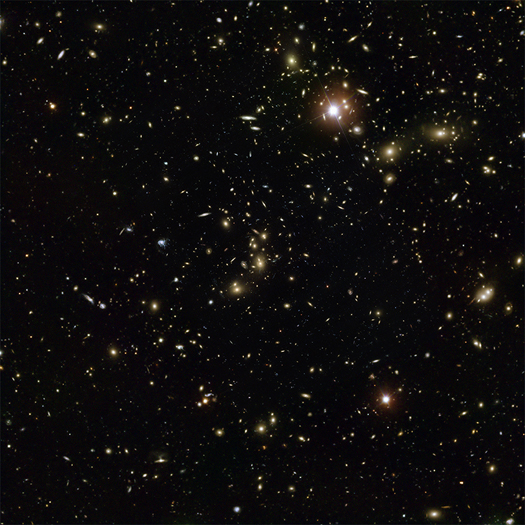
\includegraphics[width=\linewidth]{Images/Chapter3/a2744_w33.jpg}
        \caption{Optical}
        \label{fig:hubble_abell2744}
    \end{subfigure}
    \hspace{2mm}
    \begin{subfigure}{0.31\textwidth}
        \centering
        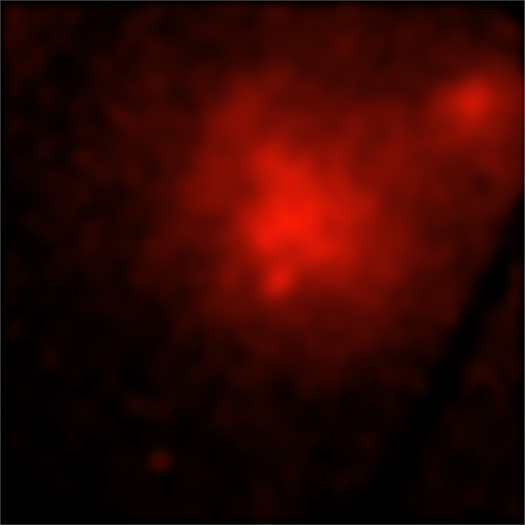
\includegraphics[width=\linewidth]{Images/Chapter3/a2744_w22.jpg}
        \caption{X-ray}
        \label{fig:chandra_abell2744}
    \end{subfigure}
    \hspace{2mm}
    \begin{subfigure}{0.31\textwidth}
        \centering
        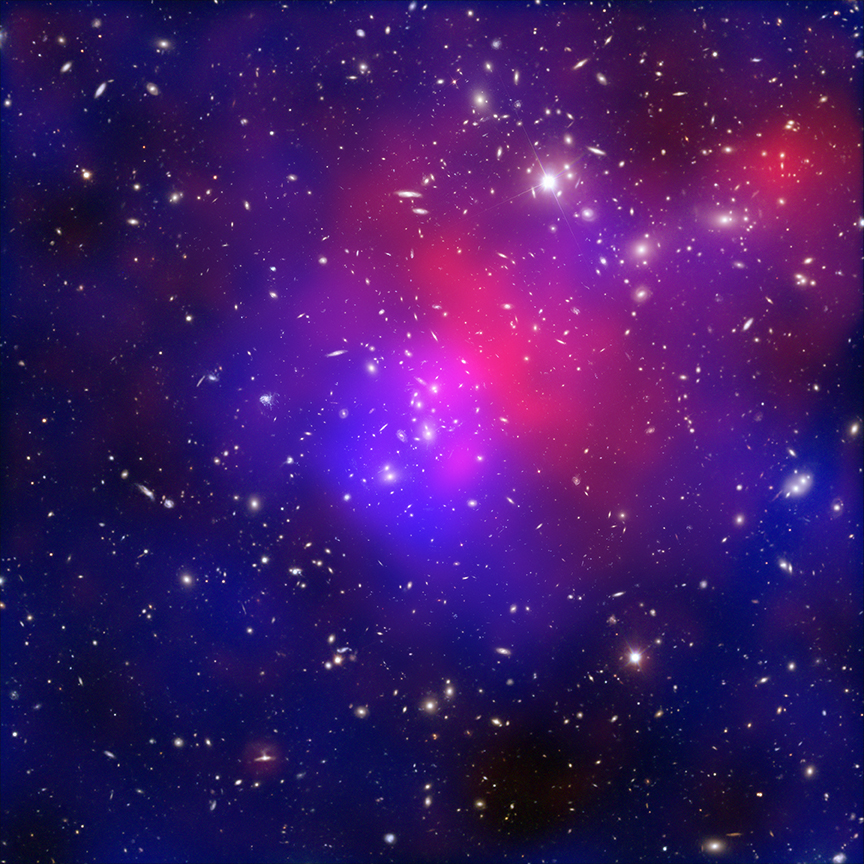
\includegraphics[width=\linewidth]{Images/Chapter3/a2744.jpg}
        \caption{Combined with DM}
        \label{fig:combined_abell2744}
    \end{subfigure}
    \caption[Multi-wavelength observations of galaxy cluster Abell 2744]{
        Multi-wavelength observations of the galaxy cluster Abell 2744. 
        \textbf{Left:} Optical image taken by Hubble Space Telescope and VLT. 
        \textbf{Center:} X-ray image by Chandra X-Ray Observatory. 
        \textbf{Right:} Combined images, the blue zone is the distribution of dark matter according to Hubble's data. Credits \cite{chandra-a2744}.
    }
    \label{fig:abell2744_multiwavelength}
\end{figure}
As we can easily see in fig. \ref{fig:abell2744_multiwavelength}, galaxies are only a small part of the cluster.\\ 
About $5\%$ of the entire mass is formed by galaxies (ref. \cite{Gonzalez_2007}), another $10\%$ is formed by gas (ICM) and about $80\%$ by dark matter.

\subsection{Intra Cluster Medium (ICM)}
The Intracluster Medium (ICM) is hot, diffuse gas that permeates the space between the galaxies in the cluster itself (ref. \cite{CavaliereGurskyTucker1971}, \cite{Forman_Kellogg_Gursky_1972}). It constitutes the most important part of the baryonic matter, with an average abundance of 10\%.
Initially, it was thought that the presence of this gas could exclude the need to introduce dark matter, but even adding its contribution does not amount to the total mass of the cluster calculated through the virial theorem or the study of the X-ray radiation emitted by the ICM itself.
Due to its high temperature ($10^7 - 10^8 \; K$), the ICM can be considered completely ionized. Its density is very low, about $10^{-4} - 10^{-2} \text{ cm}^{-3}$. It contains heavy elements like Carbon, Oxygen, and Iron. This composition indicates the presence of phenomena such as supernovae that generate and distribute these elements.
Its emission on the electromagnetic spectrum is located in the X-ray region. It is generated by the interaction of free electrons (the ICM can be considered like an ionized plasma) and atomic nuclei with thermal bremsstrahlung.\\ 
The ICM is also responsible for the Sunyaev-Zel'dovich effect (or SZ effect), photons of CMB that are crossing the cluster interacting with ionized ICM through an inverse scattering Compton with free high-energy electrons, this phenomenon causes a distortion in the CMB (ref. \cite{SZ_effect}).

In a relaxed cluster, the radial distribution for gas may be described by the beta model:
\begin{equation} \label{gas fit}
    n(r) = \rho_s \qty[1+\qty(\frac{r}{r_c})^2]^{-\frac{3}{2} \beta},
\end{equation}
where $\beta$ is an index that describes how the gas density decreases as a function of radius and $r_c$ is the core radius. With $\beta = 2/3 \sim 0.67$ we have the King profile (ref. \cite{King_profile}).

\subsection{Brightest Cluster Galaxy (BCG)}
In almost all galaxy clusters, there is a giant galaxy that dominates the cluster, typically a giant elliptic galaxy with an extended and diffused halo. This galaxy is also called Brightest Cluster Galaxy (BCG). These galaxies are very massive, with mass over $10^{12} \; M_\odot$, and also their contribution to the cluster luminosity is very important. Most of the time this galaxy is an elliptical cD galaxy (where "D" stands for "diffuse") as reported in ref. \cite{Galaxy-Formation-and-Evolution}.
Due to this morphology, its surface brightness profile is well described by the Vaucouleurs profile (ref. \cite{de_Vaucouleurs_1948}), a particular case of the Sersic profile (ref. \cite{Sersic_model_1963}). However, this last one is very difficult to deproject, so we can use more simply the Jaffe luminosity profile (ref. \cite{Jaffe_profile_1983})
\begin{equation}
    L_J (r) = L_{source} \frac{r}{r_J} \qty(1+\frac{r}{r_J})^{-1},
\end{equation}
assuming that the luminosity profile follows the mass profile it's possible to define a mass profile for the BCG as
\begin{equation}
    M (r) = M_{*} \frac{r}{r_J} \qty(1+\frac{r}{r_J})^{-1} = L_{source} X_L,
\end{equation}
where $X_L$ is the mass-luminosity ratio measured in $M_\odot/L_\odot$.
This profile has a density profile written in the following way
\begin{equation} \label{jaffe profile}
    \rho (r) = \frac{\rho_J}{\qty(\frac{r}{r_J})^2 \qty(1+\frac{r}{r_J})^2},
\end{equation}
where $r_J$ is Jaffe's radius and $\rho_J = \frac{M_*}{4\pi r_J^3}$ with $M_*$ the total stellar mass in the BCG.\\
This profile will be used in Chapter \ref{Capitolo4} to fit the contribution to the mass cluster given by the BCG.\\
In dynamically relaxed systems, the BCG is usually located close to the center defined either by the X-ray peak of the intra cluster medium gas or by the mass peak reconstructed from gravitational lensing (ref. \cite{Stellar_mass–halo_mass_relation_for_the_brightest_central_galaxies_of_X-ray_clusters_since_z_0.65}).\\
However, recent X–ray/optical studies show that this is not universal:
up to $\sim$ 40\,\% of BCGs are displaced from the X–ray peak by
tens of kiloparsecs, with a median separation of $\sim$ 15 kpc and
extreme cases beyond 100 kpc (ref. \cite{De_Propris_2020}).\\
The origin of BCGs is still debated. Early studies proposed a single–process such as only the BCG cannibalism mechanism (ref. \cite{BCG_Cannibalism_Ostriker_&_Hausman_1977}) or only the cooling flows (ref. \cite{Cooling_flow_Cowie_&_Binney_1977}), but more recent work indicates that BCGs are more likely to form through a multi–stage process.
At high redshift, the bulk of the primary stellar mass is assembled in short, intense episodes of star formation and only later does the galaxy grow mainly through mergers with satellites that spiral toward the cluster center during its evolution.

\subsection{Galaxies}
Like we said before, galaxies form only about 5\% of the entire mass of a galaxy cluster, but this is not a good reason to ignore them. In fact, galaxies can be used as tracers to determine the mass of the cluster itself through dynamical analyses (this is exactly what we will do in the next Chapter \ref{Capitolo4}).\\
There are several types of galaxies that can be divided in few groups in function of their colors and morphology. From the morphological point of view, according to Hubble classification, galaxies have 3 principal shapes: elliptic, spiral and irregular.
The age of a galaxy is connected to  its color, as the presence of a large number of red stars indicates that the galaxy is old (red stars live more than blue stars); on the opposite, a large number of blue stars indicates a young galaxy.

Galaxies are also divided into two sequences defined by a number of characteristic properties. Early type galaxies are characterized by elliptical and lenticular shape, old and red stars, poor in gas, a low star formation rate (SFR). On the other hand, late type refers to spiral and irregular galaxies, with young and blue stars, rich in gas and active SFR.\\It is important to note that in Hubble’s scheme “early type” and “late type” are morphological labels, not age indicators. In the nearby Universe, early-type galaxies generally host older stellar populations and late-type galaxies younger ones, but the terms themselves do not encode age; they persist as a historical holdover from Hubble’s original classification.\\
%To study the distribution of galaxies in clusters it is useful to separate galaxies into two classes: red, bulge-dominated, high-mass, passively-evolving galaxies and, blue, disk-dominated, low-mass, star-forming (SF hereafter) galaxies. In ref. \cite{Annunziatella_2014} is described the dependence of the distribution of galaxies as a function of radius from the center of the cluster. To do this, the cluster MACS 1206, was used in the analyses. What it is possible to find is that the shape of the star mass function (SMF hereafter) of SF galaxies is independent from the environment or clustercentric radius. Instead, the shape of the SMF of passive galaxies depends on the environment. In the core, massive passives dominate and light passives and SF are lacking; towards the outside, SF and low mass passives increase.\\ In the end, the stellar mass density profile is significantly more concentrated than the number density.\\
In galaxy clusters, the majority of member galaxies are early type systems. These galaxies are typically red, bulge dominated, massive and characterized by old stellar populations with little or no star formation. On the other hand, late type galaxies are bluer, disk dominated, gas rich, with a high star formation rate but they are a smaller fraction within clusters compared with the entire population.
In particular, ref. \cite{Annunziatella_2014} studied the galaxy population of the massive cluster MACS 1206 as a function of radius from the center of the cluster. What it is possible to find is that the shape of the star mass function (SMF hereafter) of SF galaxies is independent from the environment or clustercentric radius. Instead, the shape of the SMF of passive galaxies depends on the environment. In the core, massive passives dominate and light passives and SF are lacking; towards the outside, SF and low mass passives increase.\\ These general "properties" are well illustrated in figure  \ref{Galaxy distribution}.\\ In the end, the stellar mass density profile is significantly more concentrated than the number density.\\

In a relaxed cluster, galaxies are characterized by the distribution of cluster galaxy velocities and positions.
The projected number density of galaxies typically follows the cluster's mass density distribution; highest in the central regions and decreasing with cluster radius. Some observations show that the distribution can be described by an NFW profile with early-type galaxies more concentrated toward the center than late-type (ref. \cite{CLASH-VLT:-The-Inner-Slope-of-the-MACS-J1206.2-0847-Dark-Matter-Density-Profile}).
The radial velocity of individual galaxies is distributed around a mean in a Gaussian function (ref. \cite{Sarazin2002}). In a first approximation, this distribution is usually adopted to simplify the problem, but many studies have demonstrated that this is a very good approximation consistent with observations \footnote{This is true if the velocity is not to high.} (ref. \cite{The_Velocity_Distribution_of_Galaxies_in_Clusters_1977}).
Anyway, the dispersion velocity in a cluster decreases from the center to the outer region.
\begin{figure}[h!]
\centering
    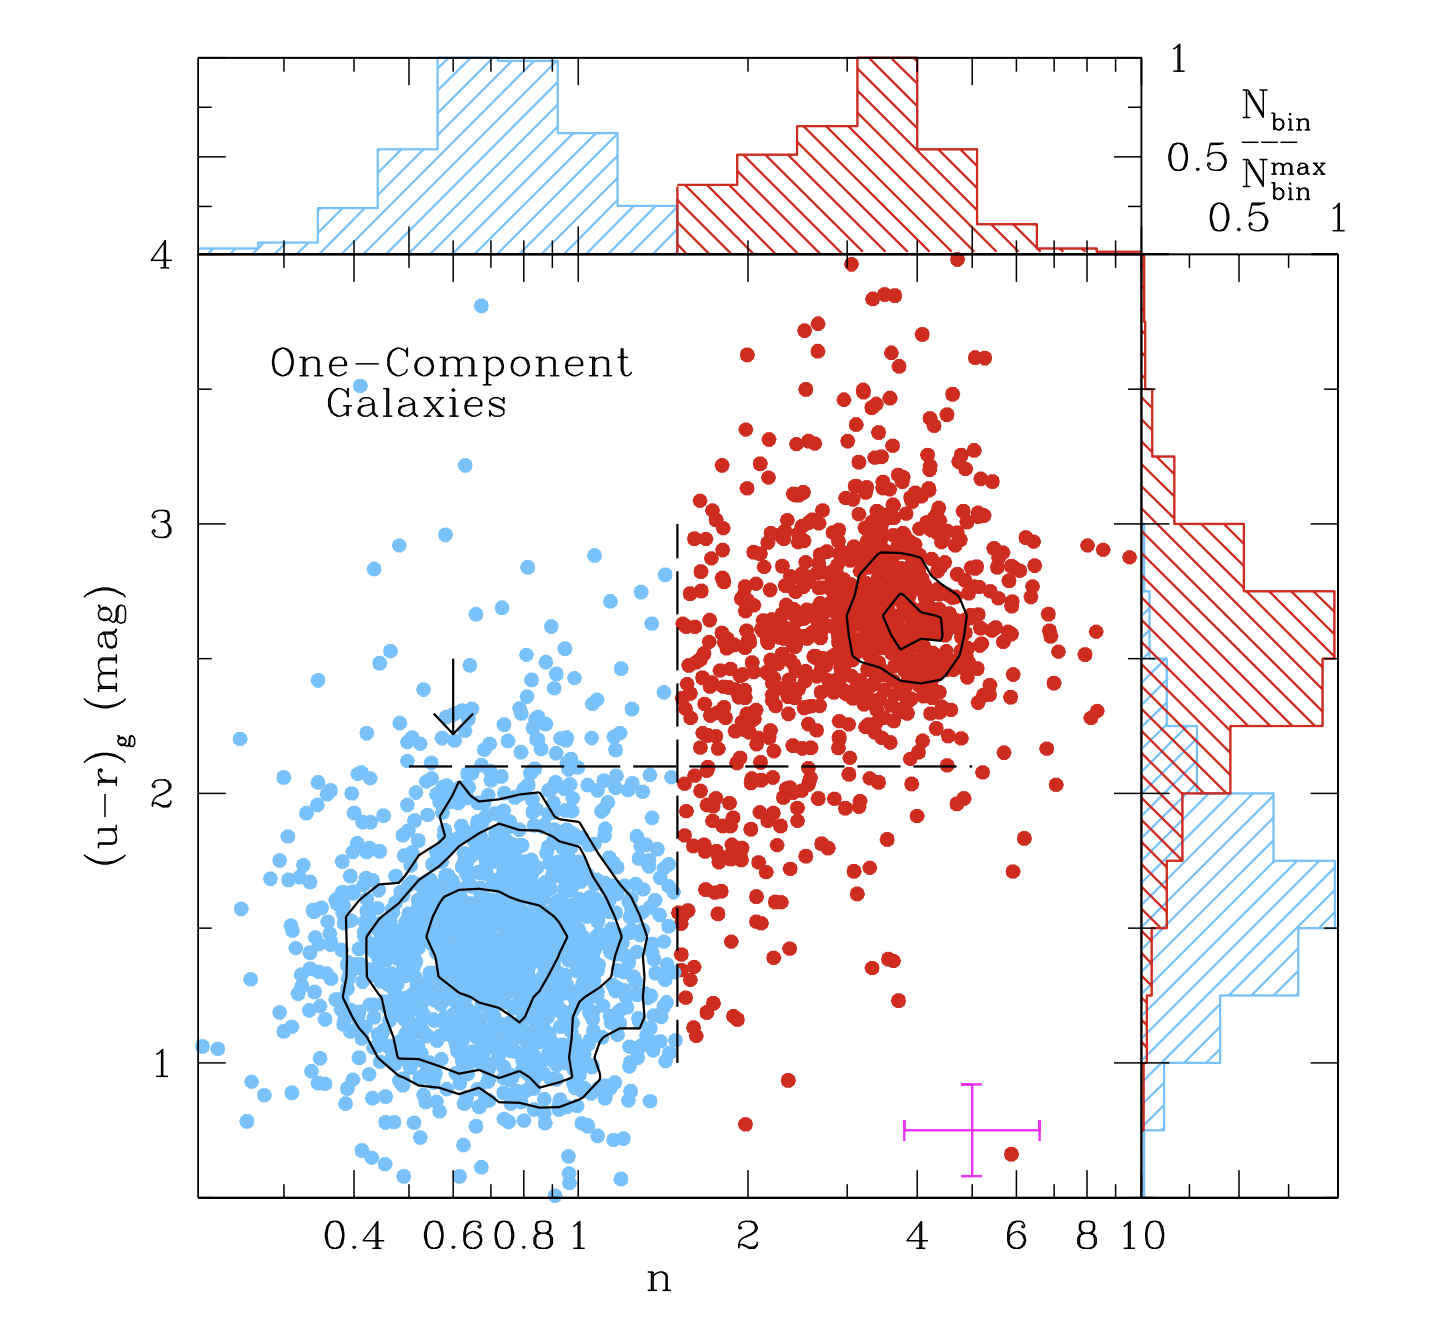
\includegraphics[width=0.47\linewidth]{Images/Chapter3/Galaxy distribution.png}
    \caption[Galaxy distribution]{Figure shows the global-Sérsic index distribution. Two distinct peak clearly emerge: a red highly concentrated sequence populated by elliptical galaxies and a blue diffused sequence populated by disk systems. Disk only systems are represented by filled, blue circles and elliptical systems by filled, red circles. This bimodality reflects the fundamental separation between early type and late type galaxies. Credits \cite{Cameron_2009}.}
\label{Galaxy distribution}
\end{figure}

\section{Mass reconstruction}
In Chapter \ref{Dark matter properties}, we have seen an application of the virial theorem to determine the mass of a galaxy. This is not the only possible method; other important and useful approaches include analyzing the light emitted by galaxies, studying their dynamical properties, or observing their distortion through gravitational lensing.

\subsection{Mass reconstruction from X-ray observations}
We can imagine a galaxy cluster as a system of gas in hydrostatic equilibrium, within a spherical and symmetric environment at constant temperature.
Under these hypothetical conditions, it is possible to determine the total mass \footnote{Obviously, the mass is the combination of dark and baryonic matter.} distribution in the cluster.
The condition for hydrostatic equilibrium can be written as follows:
\begin{equation}\label{hydrostatic equilibrium condition}
\frac{dp}{dr} = -\frac{GM(<R) \rho}{r^2},
\end{equation}
where $\rho$ is the gas density, $p$ is the pressure, and $M(<R)$ is the mass contained within radius $R$ in the cluster.
Due to the high temperature of the gas, we can use the ideal gas law expressed in terms of density:
\begin{equation}\label{x-ray pressure}
    p = \frac{kT \rho}{\mu m_H},
\end{equation}
where $k$ is the Boltzmann constant, $\mu$ is the mean molecular weight of gas. We also assume that a large amount of gas is formed by hydrogen.
Now we can differentiate \eqref{x-ray pressure} and equate it with the hydrostatic equilibrium condition \eqref{hydrostatic equilibrium condition} and find:
\begin{equation}
    \frac{kT}{\mu m_H}\qty(\frac{1}{\rho} \frac{d\rho}{dr} + \frac{1}{T}\frac{dT}{dr}) = - \frac{GM(<R)}{r^2},
\end{equation}
and from this find the mass
\begin{equation}
    M(<R) = -\frac{kTr^2}{G \mu m_H} \qty[\frac{d\log\rho}{dr} + \frac{d\log T}{dr}].
\end{equation}
Where $M(<R)$ is the cumulative mass within $R$ radius. This is the result reported in ref. \cite{X-Ray_mass_determination_M87} and \cite{PhDPizzuti}. 
With this equation, if it is possible to measure the temperature of gas (for example, with an X-ray telescope) and the total visible mass, it's possible to find the total mass of the cluster and then the percentage of dark matter.

\subsection{Mass reconstruction with lensing}

In 1919, Arthur Eddington demonstrated the General Relativity theory through the deflection of the light of some stars following the passage of the latter in the gravitational field produced by the Sun (ref. \cite{Eddington_GR}).
A similar method can be applied to galaxy clusters, providing a wonderful way to study and calculate the mass contained in a galaxy. Light travels through empty space and it is deflected by the presence of massive objects such as galaxy clusters.\\

In General Relativity, propagation of light subject to a gravitational potential $\Phi$ can be described as in a medium with a refractive index
\begin{equation}
    n \sim 1-\frac{2\Phi}{c^2}.
\end{equation}
The deflection angle is proportional to the transversal gradient of the index $n$ that light meets during the path. Indicating with $\vec{\Tilde{\alpha}}$ the angle of deflection and with $\nabla_{\perp}n$ the gradient of $n$ perpendicular to the direction of propagation, we can write in general:
\begin{equation}\label{potential lensing path equation}
    \vec{\Tilde{\alpha}} = - \int \nabla_\perp n \;dl \approx \frac{2}{c^2} \int \nabla_\perp \Phi dl,
\end{equation}
where the integral is along the way of the light ray through the gravitational field. The minus sign indicates that the deviation is toward the region with higher $n$, or deeper gravitational potential (ref. \cite{Lectures_Gravitational_Lensing}).
Now we can apply the upper formula \eqref{potential lensing path equation} to calculate the deflection by a point mass $M$.\\ Let's consider a light ray which passes at a certain impact parameter $\xi$ (minimum distance between the light ray and mass) from the mass $M$ and let's set the $z$-axis as the direction of propagation of non-deflected light and $\vec{\xi}$ a bidimensional vector on the perpendicular plane with respect to $z$-axis. In this case, with a point mass, the deflection angle is simply given by
\begin{equation}\label{alpha reduced}
    \Tilde{\alpha} = \frac{4GM}{c^2 \xi},
\end{equation}
where $M$ is the mass of the deflector body, $\xi$ is the impact parameter\footnote{See ref. \cite{Lectures_Gravitational_Lensing} for more details.}.
However, most of the time, mass is not a single dot but a continuous distribution of mass. In this case, we make a reasonable approximation: if the region where the mass is concentrated is much smaller than the distance between the source and the observer, we can imagine that the deflection essentially occurs in a single “layer” around the plane of the lens (see e.g. ref. \cite{PhDPizzuti}).\\
We then introduce a coordinate system on the plane of the lens, perpendicular to the line of sight and we denote with $\Sigma(\vec{\xi})$ the surface mass density (or, in other words, the integrated mass along the line of sight at an arbitrary point $\vec{\xi}$ of the lens plane).\\
The deflection angle can be rewritten in terms of position as follows
\begin{equation}
    \vec{\Tilde{\alpha}} (\vec{\xi}) = \frac{4G}{c^2} \int \frac{\Sigma (\vec{\xi'})(\vec{\xi} - \vec{\xi'})}{|\vec{\xi} - \vec{\xi'}|} d^2 \xi '.
\end{equation}
To understand how the deflection of light, due to a large mass, is translated in alternate positions and shapes, it's important to analyze the geometry of the source-lens-observer system.\\
Now let's consider a lighting source (S) behind the lens (L) as compared to an observer (O).\\
\begin{figure}[h!]
\centering
    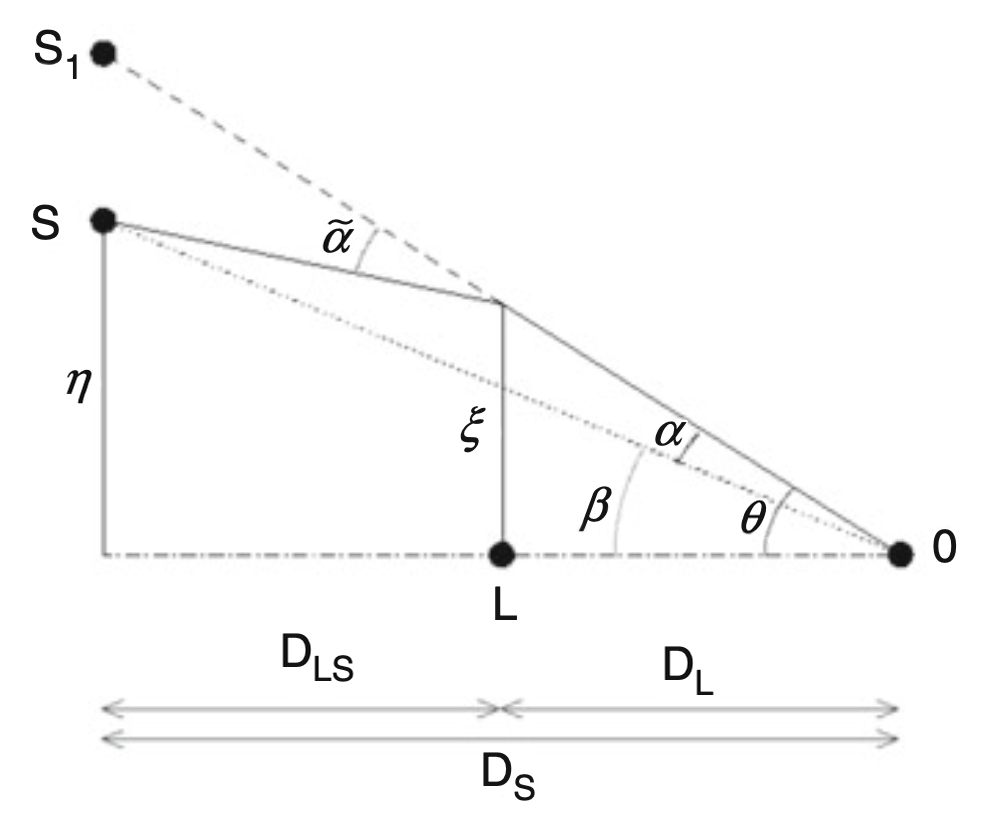
\includegraphics[width=0.50\linewidth]{Images/Chapter3/Lensing schema.png}
    \caption[Scheme of gravitational lensing]{Scheme of gravitational lensing. S, S$_1$, L and O are respectively the real position of the source, the position of image of source from the view of the observer, the lens and the finally the observer. $\xi$ is the impact parameter (minimum distance between deflected light ray and body that produce lens). $\vec{\Tilde{\alpha}}$ is the deflected angle and $\vec\alpha$ the reduced deflected angle. In the end, $D_{LS}$, $D_L$ and $D_S$ are respectively the distance of lens-source plane, distance lens-observer plane and distance source-observer plane. Credits \cite{Longair}.}
\label{Scheme of gravitational lensing}
\end{figure}In the absence of the lens, the observer can see the source with an angle $\beta$ as compared to the optic axis lens-observer; in the presence of the lens, the light ray is deflected with an angle $\vec{\Tilde{\alpha}}$ reaching the observer with an effective angle $\vec{\theta}$. Now we can introduce the reduced angle $\vec{\alpha}$ that can be written, with some geometry, as
\begin{equation}\label{alpha_definition}
    \vec{\alpha} = \frac{D_{LS}}{D_S} \vec{\Tilde{\alpha}},
\end{equation}
where $D_{LS}$ is the projected distance between the lens and source, while $D_S$ is the projected distance of the source from the observer.
This reduced angle $\vec\alpha$ represents the actual angular displacement of the source position as seen by the observer, taking into account that the deflection occurs at the plane of the lens and “projecting” this deflection up to the source plane.
The fundamental equation of the gravitational lensing allows us to connect angles in the optic scheme below
\begin{equation}\label{lensing equation}
    \vec\beta = \vec\theta - \vec\alpha(\vec{\theta}).\footnote{This relation can be founded by $\vec\theta D_S = \vec\beta D_S + \vec{\Tilde{\alpha}} D_{LS}$ if corners are enough small.}
\end{equation}
Due to the dependence of the position of the objects, the deflection angle can be variable; for example, if $\xi$ is smaller, the deflection will be bigger. It is also very important to notice that there are a few solutions for this equation, so it is possible to have more images for a single source.\\ 
We have defined $\vec\alpha$ \eqref{alpha_definition} and reduced angle \eqref{alpha reduced} before, so combining all of them in the last one \eqref{lensing equation} we obtain
\begin{equation}
    \vec\beta = \vec\theta - \frac{D_{LS}}{D_S} \vec{\Tilde{\alpha}}.
\end{equation}
For a lens with circular symmetry and mass given by fixed uniform surface density we can write $M(\xi) = \Sigma \pi \xi^2$ (mass in a circle with radius $\xi$)
\begin{equation}
    \alpha = \frac{D_{LS}}{D_S} \Tilde{\alpha} = \frac{D_{LS}}{D_S} \frac{4 \pi G\Sigma(\xi)}{\xi c^2},
\end{equation}
It is also possible to introduce a critical surface density
\begin{equation}
    \Sigma_{crit} = \frac{D_S}{D_{LS} D_L} \frac{c^2}{4 \pi G}.
\end{equation}
Furthermore $\xi = D_L \theta$ and substituting all into the lens equation, we found a linear formula
\begin{equation}
    \beta = \theta - \frac{4 \pi G \Sigma(\theta)}{c^2}\frac{D_L D_{LS}}{D_S}\theta.
\end{equation}
A fascinating phenomenon happens when the source, lens and observer are aligned. In this case $\beta = 0$ and the previous equation gives life to the Einstein ring (see fig. \ref{fig:Einstein ring by Euclid})
\begin{equation}
    \theta_E = \sqrt{\frac{4GM(\theta_E)}{c^2} \frac{D_{LS}}{D_L D_S}}.
\end{equation}
This is used to determine two kinds of regimes: strong lensing ($\theta < \theta_E$) and weak lensing ($\theta > \theta_E$).

\subsubsection{Weak lensing}
The weak lensing regime occurs when the lens has a surface density lower than the critical one ($\Sigma < \Sigma_{crit}$) over the entire field considered, so that no multiple images or very pronounced arches are formed.\\ Individual sources undergo changes too small to be distinguished from the intrinsic variability of galaxies' shapes and brightnesses. However, by statistically analyzing a large number of background sources, it is possible to reveal a consistent correlation in the distortions: typically, background galaxies tend to be stretched tangentially around the lens center with the semi-major axis of the image ellipse oriented perpendicular to the radius joining it to the lens center (ref. \cite{2024darkmatter}).\\ This phenomenon can be easily seen in an illustrative example in fig. \ref{fig:weak lensing}.
\begin{figure}[h!]
    \centering
    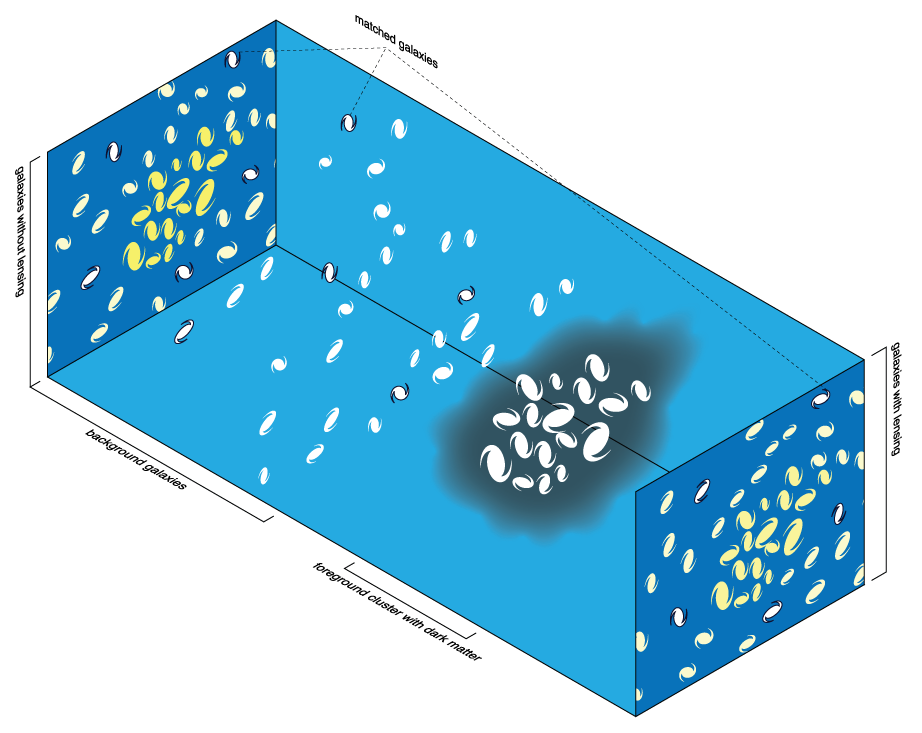
\includegraphics[width=0.5\linewidth]{Images/Chapter3/Gravitational-weak-lensing-3d.png}
    \caption[Weak lensing]{Three-dimensional representation of weak lensing: a foreground galaxy cluster weakly distorts the images of background galaxies along the line of sight. On the left, the same galaxies are shown without lensing; on the right, the lensed images appear slightly stretched and tangentially aligned around the cluster's mass. Credits \cite{Sachs2008WeakLensing3D}.}
    \label{fig:weak lensing}
\end{figure}

\subsubsection{Strong lensing}
When the effect of a lens is strong enough to produce multiple images or easily visible macroscopic distortions of a single background source. It normally occurs when the surface density is greater than the critical one ($\Sigma > \Sigma_{crit}$).\\
If the alignment is almost perfect or if the source is very large, bright arches or even Einstein rings can form.\\ Sometimes, the magnification can be so strong to allow us to see objects too faint, this creating a giant natural gravitational space telescope giving us several data.
\begin{figure}[h!]
    \centering
    \includegraphics[width=0.55\linewidth]{Images/Einstein ring by Euclid.pdf}
    \caption[Einstein ring around NGC 6505 photographed by Euclid]{A wonderful example of strong lensing: Einstein ring around NGC 6505, photographed by the Euclid Space Telescope. The large background image shows the full cluster with the Einstein ring structure clearly visible. The inset panel (right-side) provides a close-up view of the ring. Figure 1 in ref. \cite{Einstein_ring_Euclid_image}.}
    \label{fig:Einstein ring by Euclid}
\end{figure}

\clearpage

\section{Mass reconstruction with kinematics of member galaxies}
As seen in Chapter \ref{Dark matter properties}, it is possible to use the expressions for galaxy velocities to reconstruct the mass of a cluster. We will now introduce and explain some fundamental equations, like the Vlasov and Jeans equations, for the next chapter.
Galaxy clusters are very different from gases, where particles collide with each other. In fact, here the predominant interaction is gravitational, which acts on large scales and which strength intensifies as galaxies approach each other. For this reason, it will be useful and sufficient to consider our system as a collection of collisionless particles.

\subsection{Vlasov equation}

The Vlasov equation describes the evolution of a self-gravitating system of collisionless particles in terms of the distribution of particles in position-velocity phase space ($\Vec{x}, \Vec{v}$). Conceptually, it imposes the conservation of particle density in phase space along the motion; in absence of collisions, particles move so that the distribution, described by a function $f(\Vec{x}, \Vec{v}, t)$, remains constant along a phase trajectory.
The flow of particles in phase space then behaves like an incompressible fluid as long as the interactions of the particles are negligible. For the purposes of discussion on galaxy clusters, this remains a very good approximation until relaxation times due to close encounters between particles are comparable with the age of the universe. A cluster can then be treated as a collisionless system in which the dynamics are governed by a gravitational potential generated by the mass distribution.

Now, with the distribution function $f(\Vec{x}, \Vec{v}, t)$ we construct the number of particles in a volume element of the phase space.
\begin{equation}
    dN = f(\Vec{x}, \Vec{v}, t) d^3x d^3v.
\end{equation}

The time evolution of $f$ is obtained by imposing continuity in phase space. Consider a six-component state vector (three related to position and three related to velocity).
\begin{equation}
    w = (\Vec{x},\Vec{v}),
\end{equation}
its equation of motion will be
\begin{equation}
    \dot{w} = (\dot{\Vec{x}}, \dot{\Vec{v}}) = (\Vec{v}, -\nabla \Phi),
\end{equation}
where $\Phi$ is the gravitational potential that satisfies the usual Poisson equation.
Putting everything together, phase-space continuity is written as the following equation:
\begin{equation} \label{vlasov continuità}
    \frac{\partial f}{\partial t} + \sum_{i=1}^{6} \frac{\partial (f \dot{w}_i)}{\partial w_i} = 0,
\end{equation}
Now, since the gravitational potential does not explicitly depend on $\vec{v}$ and that $\Vec{x}$ and $\Vec{v}$ are independent variables, it is possible to integrate the eq \eqref{vlasov continuity} and obtain the Vlasov equation

\begin{equation}\label{vlasov equation}
    \frac{\partial f}{\partial t} + \sum_{j=1}^{3} \Big( v_j\frac{\partial f}{\partial x_j} - \frac{\partial \Phi}{\partial x_j}\frac{\partial f}{\partial v_j} \Big) = 0,
\end{equation}
or more conveniently written thanks to the convective derivative
\begin{equation}
    \frac{Df(\Vec{x}, \Vec{v},t)}{dt} = 0,
\end{equation} 
highlighting that the derivative of $f$ along the motion is zero and that consequently the density of the particles (equivalently to the incompressible fluid) is conserved.

\subsection{Jeans equation}
The Jeans equation is obtained as the moment of the Vlasov equation and allows us to connect dynamical observable properties such as mean velocity, dispersion velocities and their anisotropies with gravitational potential. From a certain point of view, the Jeans equation is analogous to the Euler equation for a self-gravitating fluid where the pressure is replaced by the dispersion of velocities.

Defines itself the spatial density of particles $\nu (\Vec{x}, t)$ and the mean velocity $\Bar{v}_i (\Vec{x}, t)$ as
\begin{equation}\label{momenti}
    \nu (\Vec{x}, t) = \int f(\Vec{x}, \Vec{v}, t) d^3v \qquad \Bar{v}_i (\Vec{x}, t) = \frac{1}{\nu} \int v_i,f(\Vec{x}, \Vec{v}, t) d^3v,
\end{equation}
and, manipulating eq. \eqref{vlasov equation}, it is possible to obtain
\begin{equation}\label{equazione di continuità jeans}
    \frac{\partial\nu}{\partial t} + \frac{\partial(\nu \Bar{v}_i)}{\partial x_i} = 0,
\end{equation}
which is the continuity equation for numerical density $\nu(\Vec{x},t)$. This equation represents the conservation of the number of galaxies in a given volume and the temporal variation of $\nu$ is due to the transport of particles (galaxies in our case) through the boundaries of the volume. 
The momentum of the Vlasov equation is obtained by multiplying by $v_j$ and integrating again in the space of velocities; in this way we obtain a balance equation of the momentum quantities for a collisionless system
\begin{equation} \label{equazione primo momento}
    \frac{\partial (\nu \bar{v}_j)}{\partial t} + \frac{\partial (\nu\overline{v_i v_j})}{\partial x_i} + \nu\frac{\partial \Phi}{\partial x_j} = 0,
\end{equation}
where $\overline{v_i v_j}$ is given by
\begin{equation}
    \overline{v_i v_j} = \frac{1}{\nu} \int v_i v_j f d^3 v.
\end{equation}
Now the equation \eqref{equazione primo momento} can be manipulated; multiplying the continuity equation by $\overline{v_j}$, then we subtract from the equation \eqref{equazione primo momento} and finally, using the Leibniz rule\footnote{See ref. \cite{Rottgering2011Lecture10} for more details on calculus.}, we also introduce the velocity stress tensor $\sigma^2_{ij}$ defined as:
\begin{equation}
    \nu \sigma^2_{ij} = \nu \overline{(v_i v_j - \bar{v}_i \bar{v}_j)} = \nu[\overline{v_i v_j} - \bar{v}_i \bar{v}_j].
\end{equation}
We thus obtain the final form of the equation we are looking for, thus finding the Jeans equation. From a physical point of view, the Jeans equation relates observable dynamical quantities with gravitational potential
\begin{equation}
    \nu\frac{\partial \bar{v}_j}{\partial t} + \nu\bar{v}_i\frac{\partial \bar{v}_j}{\partial x_i} = -\nu\frac{\partial \Phi}{\partial x_j} - \frac{\partial (\nu\sigma^2_{ij})}{\partial x_i}.
\end{equation}
It is analogous to the Euler equation for a fluid.
In the left side we have the time variation of momentum of the system and its derivative in space.
In the right side, term $-\partial(\nu \sigma^2_{ij})/\partial x_i$ plays the role of a pressure gradient. The term $-\nu \partial \Phi/\partial x_j$ is instead the gravitational force (for mass unit) that tends to accelerate particles towards regions of lower potential, that is, towards higher mass concentrations.
Since the clusters are considered in spherical symmetry approximation and in dynamical equilibrium, it is convenient to project the Jeans equation along the radial direction by setting the center of the cluster as the origin and thus rewrite the Jeans equation in spherical coordinates
\begin{equation}\label{eq di Jeans in coordinate sferiche}
    \frac{d(\nu\sigma_r^2)}{dr} + \frac{\nu(r)}{r}\Big[2\sigma_r^2(r) - \sigma_\theta^2(r) - \sigma_\phi^2(r)\Big] = -\nu(r)\frac{d\Phi}{dr},
\end{equation}
where $\sigma_{r}$ is the velocity dispersion along the radial direction, $\sigma_\theta$ is the velocity dispersion along the angular direction $\theta$ and $\sigma_\phi$ is the dispersion along the angular component $\phi$.
The velocity dispersion profile is given by
\begin{equation}\label{profilo di anisotropia delle velocità}
    \beta(r) = 1 - \frac{\sigma^2_\theta + \sigma^2_\phi}{2 \sigma^2_r}.
\end{equation}
Obviously, if we are in spherical approximation, the dispersions along the tangential and altazimuth directions are equal, $\sigma_\theta = \sigma_\phi$.
The equation \eqref{profilo di anisotropia delle velocità} is thus reduced to the following
\begin{equation}
    \beta(r) = 1-\frac{\sigma^2_\theta}{\sigma^2_r}.
\end{equation}
Sign and amplitude of $\beta$ indicated whether the orbits are preferably radial or tangential.
Setting the dispersion of radial velocities equal to the tangential one ($\sigma_r = \sigma_\theta$) we will have $\beta = 0$, this leads to isotropic orbits (the radial and tangential directions are equivalent). As the radial tendency increases ($\sigma_r > \sigma_\theta$), $\beta \rightarrow 1$ thus arriving at the limit of purely radial orbits. When tangential orbits are favored instead ($\sigma_\theta > \sigma_r$), $\beta$ decreases. In the extreme limit we have ideal circular orbits with $\sigma_r \rightarrow 0$ and $\beta \rightarrow -\infty$.\\
Introducing $\beta(r)$ into spherical Jeans equation \eqref{eq di Jeans in coordinate sferiche}, this can be rewritten as:
\begin{equation}\label{Equazione di Jeans sferica}
    \frac{d[\nu(r) \sigma_r^2(r)]}{dr} + 2\beta(r)\frac{\nu(r)\sigma_r^2(r)}{r} = -\nu(r)\frac{d\Phi(r)}{dr}.
\end{equation}
This equation relates the gradient of the gravitational potential to the radial variation of velocities and to the anisotropy term. In this way, if we measure through observations the density profile $\nu(r)$ of the galaxies in the cluster, the dispersion of radial velocities $\sigma_r(r)$ and anisotropy $\beta(r)$, it is possible to determine the gravitational potential $\Phi(r)$ by solving the Jeans equation and, from this, obtain the mass density profile of the cluster.


\section{CLASH and the CLASH--VLT program}
The Cluster Lensing And Supernova survey with Hubble (CLASH) is a 524-orbit multi-cycle treasury program that observed 25 massive galaxy clusters thanks to the Hubble Space Telescope between 2010 and 2013 to determine their mass profiles through gravitational lensing (ref. \cite{Postman_2012}, \cite{clash_stsci}).
Using 16 broadband filters from the near-UV to the near-IR on the Wide Field Camera 3 (WFC3) installed during Servicing Mission 4 in May 2009 on the Hubble Space Telescope (ref. \cite{WFC3_SM4}) and on the Advanced Camera for Surveys (ACS), CLASH reaches four primary goals:
\begin{enumerate}
  \item map the dark matter distribution in galaxy clusters through strong and weak gravitational lensing;
  \item detect Type Ia supernovae out to $z \sim 2$ to measure the role of dark energy;
  \item discover highly magnified galaxies at $z > 7$;
  \item study the structure and evolution of cluster galaxies.
\end{enumerate}

To complement the Hubble survey with spectroscopic redshifts, the CLASH-VLT Large Program carried out an extensive campaign with the VIMOS spectrograph on ESO’s Very Large Telescope (VLT).  
The survey targeted 13 CLASH clusters at $0.2 < z < 0.6$, obtaining about 31\,000 spectra, with typically 500-1000 cluster members and $\sim$ 200 lensed background galaxies for each system (ref. \cite{Rosati2014_Messenger}, \cite{clashvlt_site}).
These data provide the velocity, necessary for joint lensing–dynamical mass reconstructions.\\ In the end, to obtain high definition data of the BCG, the integral field spectrograph MUSE (Multi Unit Spectroscopic Explorer) on the VLT was used, collecting a total of 25 exposures of 1800 s each in April-May 2015 and April 2016. The three-pointing mosaic covers an effective area of 2.63 arcmin$^{2}$; owing to the overlap between pointings, the central $\sim$ 0.5 arcmin$^{2}$ reaches a depth of $\sim$ 8.5 h, while the remaining area integrates for $\sim$ 4 h (ref. \cite{MUSE_Caminha_2017}).\\


\subsection{MACS 1206}
MACS 1206 (or, more precisely, MACS J1206.2-0847) is a galaxy cluster located to $z = 0.4398$ with J2000 coordinates RA $12^\text{h} 06^\text{m} 12.15^\text{s}$ and DEC $-8$° $48'3.4^"$\footnote{Where RA and DEC indicate Right Ascension and Declination respectively refered to the center of cluster.} discovered in the MAssive Cluster Survey (MACS) as reported in ref. \cite{Ebeling2009} and its mass is well determined with gravitational lensing and Chandra X-ray emission (ref. \cite{CLASH:_MASS_DISTRIBUTION_IN_AND_AROUND_MACS_J1206.2-0847_FROM_A_FULL_CLUSTER_LENSING_ANALYSIS}). 
This cluster was deeply studied during the CLASH-VLT campaign using the Hubble Space Telescope and VIMOS as previously mentioned. In order to obtain more precise data for the central region, the spectrograph MUSE was utilized to explore in detail the BCG.
MACS 1206 can be considered as an overall dynamically relaxed system, with an almost round projected matter distribution (see ref. \cite{Girardi_et_al._2015}). Based on the CLUMPS algorithm developed in ref. \cite{Biviano_CLUMPS}, 468 cluster members are identified within 2.16 Mpc. For the choice of the cluster center, the BCG center was taken as a reference (ref. \cite{Pizzuti_refracted_gravity_2025}).\\ The dispersion velocity for the BCG is obtained with the method described in ref. \cite{Sartoris_et_al._2020} and the surface  brightness profile is fitted with a Jaffe profile. The luminosity in the \textit{I}-band is $L_{BCG} = 4.92 \cdot 10^{11} \; L_\odot$ and a Jaffe radius equals 39 kpc (ref. \cite{Pizzuti_refracted_gravity_2025}). The mass of the ICM instead is taken from \cite{Ettori_2011} and \cite{CLASH-VLT:-The-Inner-Slope-of-the-MACS-J1206.2-0847-Dark-Matter-Density-Profile}. Finally, the stellar mass of member galaxies used in the next chapter for the analysis is taken from ref. \cite{Annunziatella_2014}.\\
This cluster will be examined in detail in the next chapter due to its physical properties and makes MACS 1206 a perfect object to test our theories and simulation code.

\begin{figure}
  \centering
  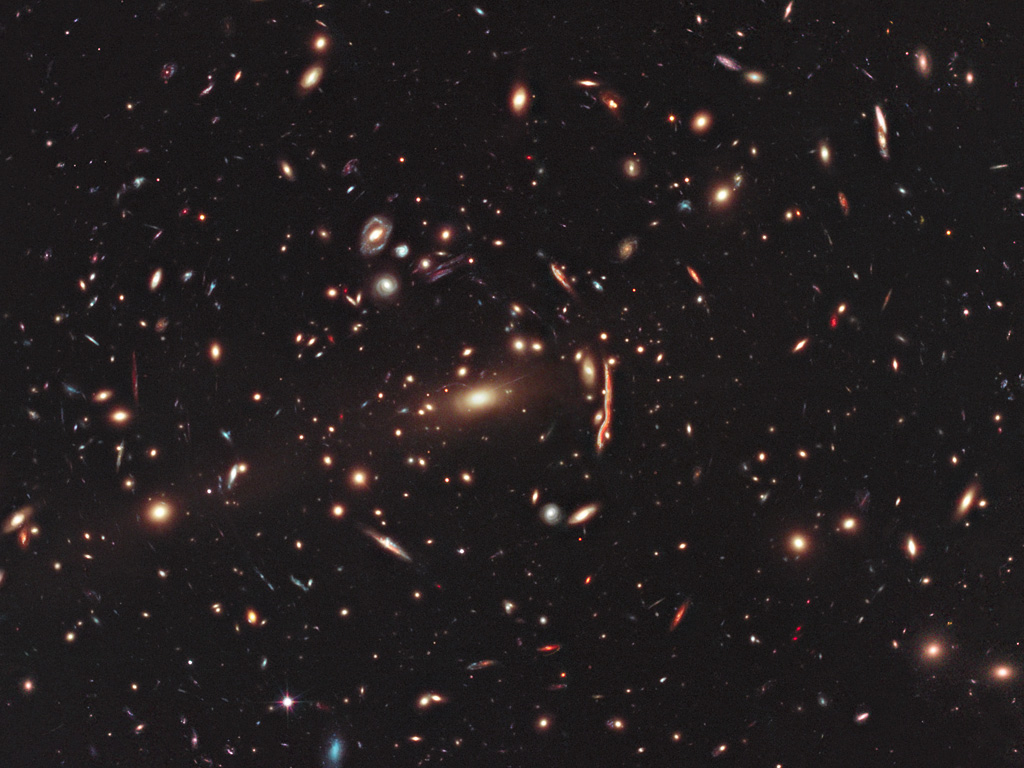
\includegraphics[width=0.62\linewidth]{Images/Chapter3/MACS1206.jpg}
  \caption[Galaxy cluster MACS 1206 by HST]{Galaxy cluster MACS J1206.2 photographed by Hubble Space Telescope. Credits \cite{MACS1206}.}
  \label{fig:macs1206}

  \vspace{8pt} % regola a gusto

  \label{tab:macs1206_parameters}
  \begin{tabular}{@{}lcc@{}}
    \toprule
    \textbf{Parameter} & \textbf{Value} & \textbf{Units} \\
    \midrule
    $z$ (redshift)           & 0.439       & -- \\
        $M_{200}$                & $1.4 \times 10^{15}$ & $M_\odot$ \\
        $r_{200}$                & 1.98        & Mpc \\
        Gas temperature $T$ & 10.5        & keV \\
        $\beta$ (profile)        & 0.67        & -- \\
        $r_c$ (core radius)   & 174.2       & kpc \\
    \bottomrule
  \end{tabular}
  \captionof{table}{Principal parameters about cluster MACS 1206}
\end{figure}